\documentclass[1p]{elsarticle_modified}
%\bibliographystyle{elsarticle-num}

%\usepackage[colorlinks]{hyperref}
%\usepackage{abbrmath_seonhwa} %\Abb, \Ascr, \Acal ,\Abf, \Afrak
\usepackage{amsfonts}
\usepackage{amssymb}
\usepackage{amsmath}
\usepackage{amsthm}
\usepackage{scalefnt}
\usepackage{amsbsy}
\usepackage{kotex}
\usepackage{caption}
\usepackage{subfig}
\usepackage{color}
\usepackage{graphicx}
\usepackage{xcolor} %% white, black, red, green, blue, cyan, magenta, yellow
\usepackage{float}
\usepackage{setspace}
\usepackage{hyperref}

\usepackage{tikz}
\usetikzlibrary{arrows}

\usepackage{multirow}
\usepackage{array} % fixed length table
\usepackage{hhline}

%%%%%%%%%%%%%%%%%%%%%
\makeatletter
\renewcommand*\env@matrix[1][\arraystretch]{%
	\edef\arraystretch{#1}%
	\hskip -\arraycolsep
	\let\@ifnextchar\new@ifnextchar
	\array{*\c@MaxMatrixCols c}}
\makeatother %https://tex.stackexchange.com/questions/14071/how-can-i-increase-the-line-spacing-in-a-matrix
%%%%%%%%%%%%%%%

\usepackage[normalem]{ulem}

\newcommand{\msout}[1]{\ifmmode\text{\sout{\ensuremath{#1}}}\else\sout{#1}\fi}
%SOURCE: \msout is \stkout macro in https://tex.stackexchange.com/questions/20609/strikeout-in-math-mode

\newcommand{\cancel}[1]{
	\ifmmode
	{\color{red}\msout{#1}}
	\else
	{\color{red}\sout{#1}}
	\fi
}

\newcommand{\add}[1]{
	{\color{blue}\uwave{#1}}
}

\newcommand{\replace}[2]{
	\ifmmode
	{\color{red}\msout{#1}}{\color{blue}\uwave{#2}}
	\else
	{\color{red}\sout{#1}}{\color{blue}\uwave{#2}}
	\fi
}

\newcommand{\Sol}{\mathcal{S}} %segment
\newcommand{\D}{D} %diagram
\newcommand{\A}{\mathcal{A}} %arc


%%%%%%%%%%%%%%%%%%%%%%%%%%%%%5 test

\def\sl{\operatorname{\textup{SL}}(2,\Cbb)}
\def\psl{\operatorname{\textup{PSL}}(2,\Cbb)}
\def\quan{\mkern 1mu \triangleright \mkern 1mu}

\theoremstyle{definition}
\newtheorem{thm}{Theorem}[section]
\newtheorem{prop}[thm]{Proposition}
\newtheorem{lem}[thm]{Lemma}
\newtheorem{ques}[thm]{Question}
\newtheorem{cor}[thm]{Corollary}
\newtheorem{defn}[thm]{Definition}
\newtheorem{exam}[thm]{Example}
\newtheorem{rmk}[thm]{Remark}
\newtheorem{alg}[thm]{Algorithm}

\newcommand{\I}{\sqrt{-1}}
\begin{document}

%\begin{frontmatter}
%
%\title{Boundary parabolic representations of knots up to 8 crossings}
%
%%% Group authors per affiliation:
%\author{Yunhi Cho} 
%\address{Department of Mathematics, University of Seoul, Seoul, Korea}
%\ead{yhcho@uos.ac.kr}
%
%
%\author{Seonhwa Kim} %\fnref{s_kim}}
%\address{Center for Geometry and Physics, Institute for Basic Science, Pohang, 37673, Korea}
%\ead{ryeona17@ibs.re.kr}
%
%\author{Hyuk Kim}
%\address{Department of Mathematical Sciences, Seoul National University, Seoul 08826, Korea}
%\ead{hyukkim@snu.ac.kr}
%
%\author{Seokbeom Yoon}
%\address{Department of Mathematical Sciences, Seoul National University, Seoul, 08826,  Korea}
%\ead{sbyoon15@snu.ac.kr}
%
%\begin{abstract}
%We find all boundary parabolic representation of knots up to 8 crossings.
%
%\end{abstract}
%\begin{keyword}
%    \MSC[2010] 57M25 
%\end{keyword}
%
%\end{frontmatter}

%\linenumbers
%\tableofcontents
%
\newcommand\colored[1]{\textcolor{white}{\rule[-0.35ex]{0.8em}{1.4ex}}\kern-0.8em\color{red} #1}%
%\newcommand\colored[1]{\textcolor{white}{ #1}\kern-2.17ex	\textcolor{white}{ #1}\kern-1.81ex	\textcolor{white}{ #1}\kern-2.15ex\color{red}#1	}

{\Large $\underline{12a_{0272}~(K12a_{0272})}$}

\setlength{\tabcolsep}{10pt}
\renewcommand{\arraystretch}{1.6}
\vspace{1cm}\begin{tabular}{m{100pt}>{\centering\arraybackslash}m{274pt}}
\multirow{5}{120pt}{
	\centering
	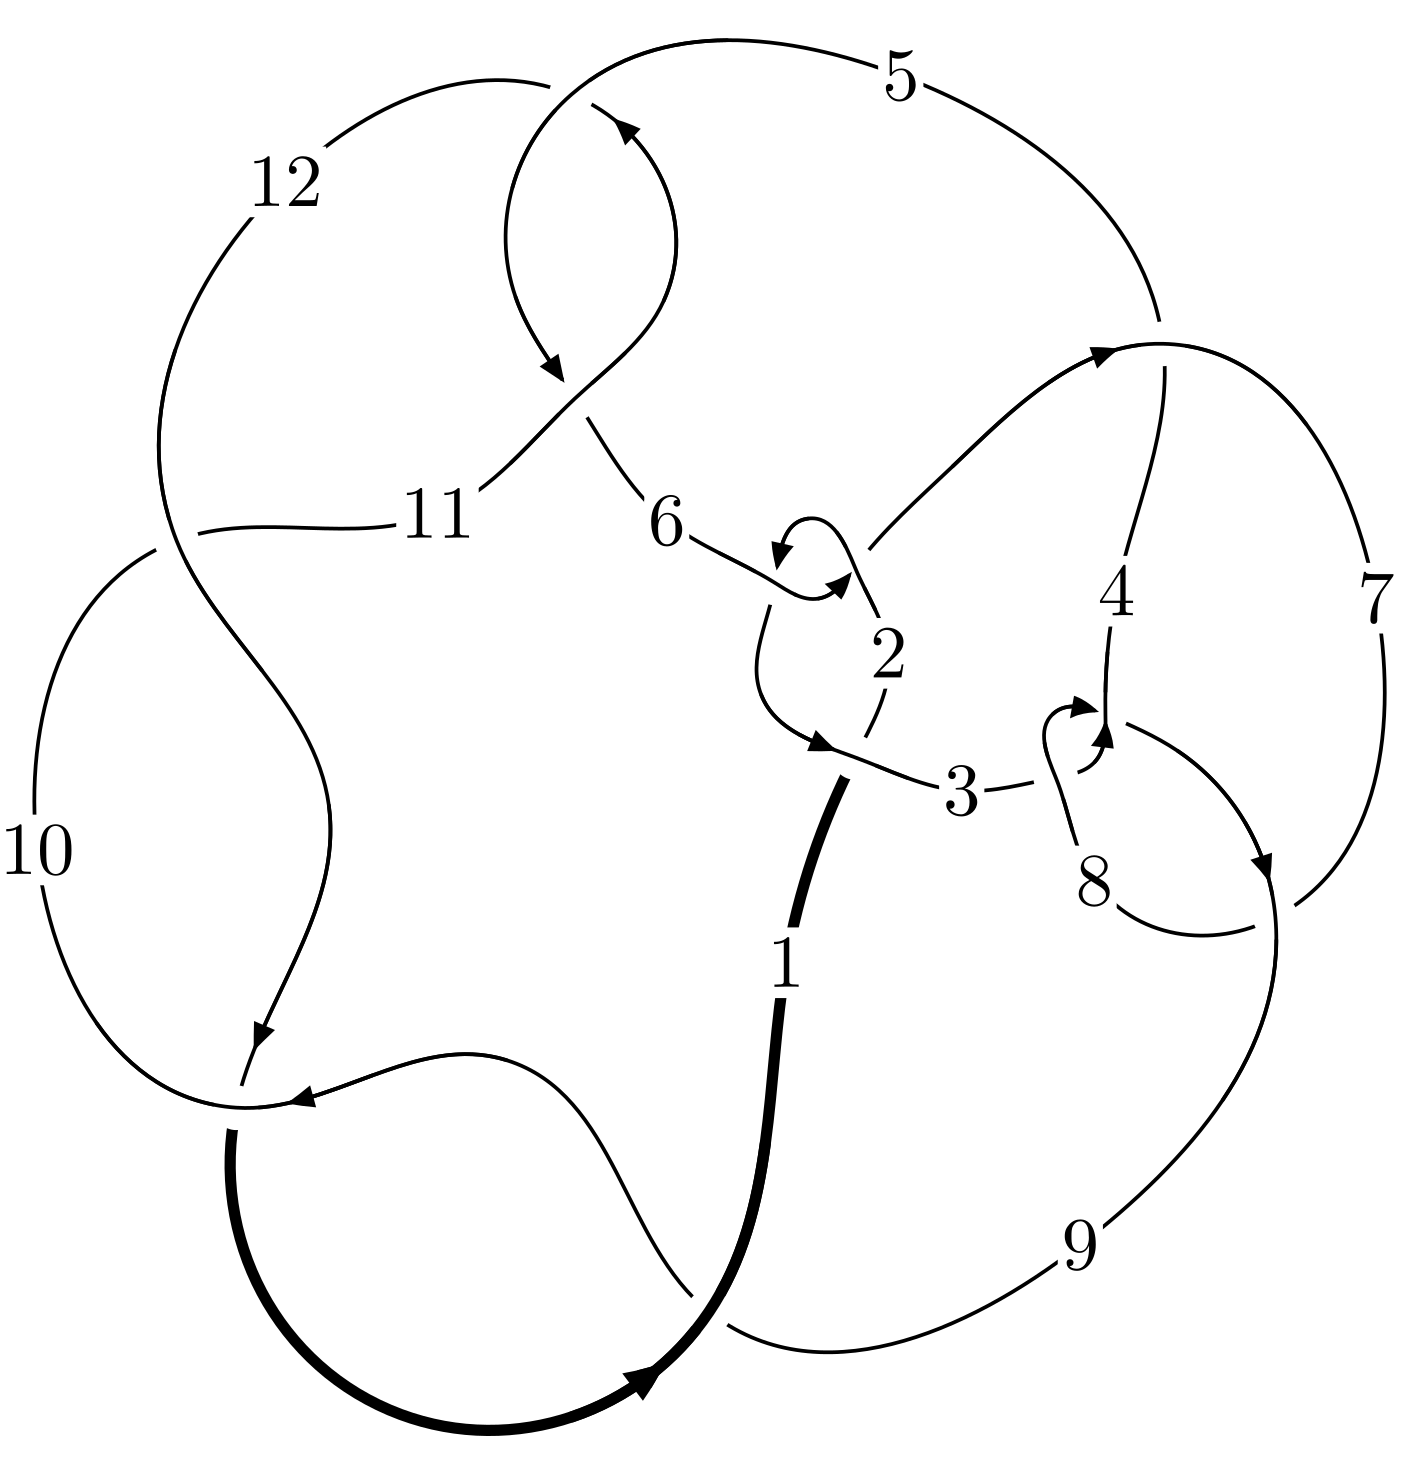
\includegraphics[width=112pt]{../../../GIT/diagram.site/Diagrams/png/1073_12a_0272.png}\\
\ \ \ A knot diagram\footnotemark}&
\allowdisplaybreaks
\textbf{Linearized knot diagam} \\
\cline{2-2}
 &
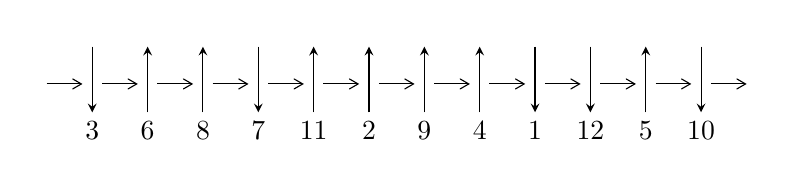
\begin{tikzpicture}[x=20pt, y=17pt]
	% nodes
	\node (C0) at (0, 0) {};
	\node (C1) at (1, 0) {};
	\node (C1U) at (1, +1) {};
	\node (C1D) at (1, -1) {3};

	\node (C2) at (2, 0) {};
	\node (C2U) at (2, +1) {};
	\node (C2D) at (2, -1) {6};

	\node (C3) at (3, 0) {};
	\node (C3U) at (3, +1) {};
	\node (C3D) at (3, -1) {8};

	\node (C4) at (4, 0) {};
	\node (C4U) at (4, +1) {};
	\node (C4D) at (4, -1) {7};

	\node (C5) at (5, 0) {};
	\node (C5U) at (5, +1) {};
	\node (C5D) at (5, -1) {11};

	\node (C6) at (6, 0) {};
	\node (C6U) at (6, +1) {};
	\node (C6D) at (6, -1) {2};

	\node (C7) at (7, 0) {};
	\node (C7U) at (7, +1) {};
	\node (C7D) at (7, -1) {9};

	\node (C8) at (8, 0) {};
	\node (C8U) at (8, +1) {};
	\node (C8D) at (8, -1) {4};

	\node (C9) at (9, 0) {};
	\node (C9U) at (9, +1) {};
	\node (C9D) at (9, -1) {1};

	\node (C10) at (10, 0) {};
	\node (C10U) at (10, +1) {};
	\node (C10D) at (10, -1) {12};

	\node (C11) at (11, 0) {};
	\node (C11U) at (11, +1) {};
	\node (C11D) at (11, -1) {5};

	\node (C12) at (12, 0) {};
	\node (C12U) at (12, +1) {};
	\node (C12D) at (12, -1) {10};
	\node (C13) at (13, 0) {};

	% arrows
	\draw[->,>={angle 60}]
	(C0) edge (C1) (C1) edge (C2) (C2) edge (C3) (C3) edge (C4) (C4) edge (C5) (C5) edge (C6) (C6) edge (C7) (C7) edge (C8) (C8) edge (C9) (C9) edge (C10) (C10) edge (C11) (C11) edge (C12) (C12) edge (C13) ;	\draw[->,>=stealth]
	(C1U) edge (C1D) (C2D) edge (C2U) (C3D) edge (C3U) (C4U) edge (C4D) (C5D) edge (C5U) (C6D) edge (C6U) (C7D) edge (C7U) (C8D) edge (C8U) (C9U) edge (C9D) (C10U) edge (C10D) (C11D) edge (C11U) (C12U) edge (C12D) ;
	\end{tikzpicture} \\
\hhline{~~} \\& 
\textbf{Solving Sequence} \\ \cline{2-2} 
 &
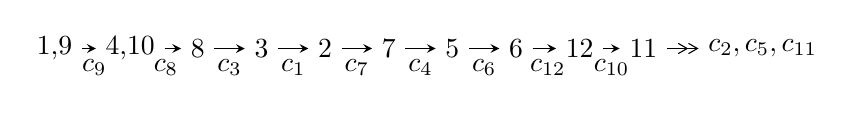
\begin{tikzpicture}[x=23pt, y=7pt]
	% node
	\node (A0) at (-1/8, 0) {1,9};
	\node (A1) at (17/16, 0) {4,10};
	\node (A2) at (17/8, 0) {8};
	\node (A3) at (25/8, 0) {3};
	\node (A4) at (33/8, 0) {2};
	\node (A5) at (41/8, 0) {7};
	\node (A6) at (49/8, 0) {5};
	\node (A7) at (57/8, 0) {6};
	\node (A8) at (65/8, 0) {12};
	\node (A9) at (73/8, 0) {11};
	\node (C1) at (1/2, -1) {$c_{9}$};
	\node (C2) at (13/8, -1) {$c_{8}$};
	\node (C3) at (21/8, -1) {$c_{3}$};
	\node (C4) at (29/8, -1) {$c_{1}$};
	\node (C5) at (37/8, -1) {$c_{7}$};
	\node (C6) at (45/8, -1) {$c_{4}$};
	\node (C7) at (53/8, -1) {$c_{6}$};
	\node (C8) at (61/8, -1) {$c_{12}$};
	\node (C9) at (69/8, -1) {$c_{10}$};
	\node (A10) at (11, 0) {$c_{2},c_{5},c_{11}$};

	% edge
	\draw[->,>=stealth]	
	(A0) edge (A1) (A1) edge (A2) (A2) edge (A3) (A3) edge (A4) (A4) edge (A5) (A5) edge (A6) (A6) edge (A7) (A7) edge (A8) (A8) edge (A9) ;
	\draw[->>,>={angle 60}]	
	(A9) edge (A10);
\end{tikzpicture} \\ 

\end{tabular} \\

\footnotetext{
The image of knot diagram is generated by the software ``\textbf{Draw programme}" developed by Andrew Bartholomew(\url{http://www.layer8.co.uk/maths/draw/index.htm\#Running-draw}), where we modified some parts for our purpose(\url{https://github.com/CATsTAILs/LinksPainter}).
}\phantom \\ \newline 
\centering \textbf{Ideals for irreducible components\footnotemark of $X_{\text{par}}$} 
 
\begin{align*}
I^u_{1}&=\langle 
-8.81378\times10^{102} u^{92}+2.11238\times10^{104} u^{91}+\cdots+4.20120\times10^{103} b+1.23437\times10^{104},\\
\phantom{I^u_{1}}&\phantom{= \langle  }1.35442\times10^{104} u^{92}-3.05756\times10^{105} u^{91}+\cdots+4.20120\times10^{103} a-2.46878\times10^{104},\;u^{93}-23 u^{92}+\cdots-7 u+1\rangle \\
I^u_{2}&=\langle 
33 a^3 u^2-12 a^3 u+42 a^2 u^2+28 a^3-76 a^2 u+165 u^2 a+66 a^2-60 a u+5 u^2+167 b+140 a-17 u-16,\\
\phantom{I^u_{2}}&\phantom{= \langle  }2 a^3 u^2+a^4-2 a^3 u+6 a^2 u^2+4 a^3-3 a^2 u+8 u^2 a+11 a^2-4 a u+3 u^2+14 a- u+7,\;u^3- u^2+2 u-1\rangle \\
\\
\end{align*}
\raggedright * 2 irreducible components of $\dim_{\mathbb{C}}=0$, with total 105 representations.\\
\footnotetext{All coefficients of polynomials are rational numbers. But the coefficients are sometimes approximated in decimal forms when there is not enough margin.}
\newpage
\renewcommand{\arraystretch}{1}
\centering \section*{I. $I^u_{1}= \langle -8.81\times10^{102} u^{92}+2.11\times10^{104} u^{91}+\cdots+4.20\times10^{103} b+1.23\times10^{104},\;1.35\times10^{104} u^{92}-3.06\times10^{105} u^{91}+\cdots+4.20\times10^{103} a-2.47\times10^{104},\;u^{93}-23 u^{92}+\cdots-7 u+1 \rangle$}
\flushleft \textbf{(i) Arc colorings}\\
\begin{tabular}{m{7pt} m{180pt} m{7pt} m{180pt} }
\flushright $a_{1}=$&$\begin{pmatrix}0\\u\end{pmatrix}$ \\
\flushright $a_{9}=$&$\begin{pmatrix}1\\0\end{pmatrix}$ \\
\flushright $a_{4}=$&$\begin{pmatrix}-3.22390 u^{92}+72.7783 u^{91}+\cdots-42.3730 u+5.87637\\0.209792 u^{92}-5.02805 u^{91}+\cdots+6.01494 u-2.93813\end{pmatrix}$ \\
\flushright $a_{10}=$&$\begin{pmatrix}1\\u^2\end{pmatrix}$ \\
\flushright $a_{8}=$&$\begin{pmatrix}2.05019 u^{92}-47.0547 u^{91}+\cdots+56.3868 u-6.05494\\-1.50087 u^{92}+34.1389 u^{91}+\cdots-17.7924 u+4.81082\end{pmatrix}$ \\
\flushright $a_{3}=$&$\begin{pmatrix}-1.01350 u^{92}+22.8011 u^{91}+\cdots+14.3088 u+1.73659\\-0.292693 u^{92}+6.74378 u^{91}+\cdots-6.73428 u+0.555834\end{pmatrix}$ \\
\flushright $a_{2}=$&$\begin{pmatrix}1.18734 u^{92}-26.3170 u^{91}+\cdots-26.1202 u+1.75144\\0.257687 u^{92}-5.95007 u^{91}+\cdots+5.55854 u-0.852157\end{pmatrix}$ \\
\flushright $a_{7}=$&$\begin{pmatrix}3.55106 u^{92}-81.1936 u^{91}+\cdots+74.1793 u-10.8658\\-1.50087 u^{92}+34.1389 u^{91}+\cdots-17.7924 u+4.81082\end{pmatrix}$ \\
\flushright $a_{5}=$&$\begin{pmatrix}0.858858 u^{92}-19.5520 u^{91}+\cdots+20.0064 u-4.50303\\-0.127780 u^{92}+2.91765 u^{91}+\cdots-0.756148 u+0.591562\end{pmatrix}$ \\
\flushright $a_{6}=$&$\begin{pmatrix}0.591562 u^{92}-13.4781 u^{91}+\cdots+17.7344 u-3.38478\\-0.180416 u^{92}+4.10757 u^{91}+\cdots-1.20608 u+0.731078\end{pmatrix}$ \\
\flushright $a_{12}=$&$\begin{pmatrix}u\\u^3+u\end{pmatrix}$ \\
\flushright $a_{11}=$&$\begin{pmatrix}u^2+1\\u^4+2 u^2\end{pmatrix}$\\&\end{tabular}
\flushleft \textbf{(ii) Obstruction class $= -1$}\\~\\
\flushleft \textbf{(iii) Cusp Shapes $= 4.26586 u^{92}-96.9345 u^{91}+\cdots+57.5150 u-12.9725$}\\~\\
\newpage\renewcommand{\arraystretch}{1}
\flushleft \textbf{(iv) u-Polynomials at the component}\newline \\
\begin{tabular}{m{50pt}|m{274pt}}
Crossings & \hspace{64pt}u-Polynomials at each crossing \\
\hline $$\begin{aligned}c_{1}\end{aligned}$$&$\begin{aligned}
&u^{93}+43 u^{92}+\cdots-3575 u-625
\end{aligned}$\\
\hline $$\begin{aligned}c_{2},c_{6}\end{aligned}$$&$\begin{aligned}
&u^{93}- u^{92}+\cdots-35 u-25
\end{aligned}$\\
\hline $$\begin{aligned}c_{3},c_{8}\end{aligned}$$&$\begin{aligned}
&u^{93}- u^{92}+\cdots+u-1
\end{aligned}$\\
\hline $$\begin{aligned}c_{4}\end{aligned}$$&$\begin{aligned}
&u^{93}-3 u^{92}+\cdots+22579 u-21009
\end{aligned}$\\
\hline $$\begin{aligned}c_{5},c_{11}\end{aligned}$$&$\begin{aligned}
&u^{93}+u^{92}+\cdots- u-1
\end{aligned}$\\
\hline $$\begin{aligned}c_{7}\end{aligned}$$&$\begin{aligned}
&u^{93}-47 u^{92}+\cdots+7 u-1
\end{aligned}$\\
\hline $$\begin{aligned}c_{9},c_{10},c_{12}\end{aligned}$$&$\begin{aligned}
&u^{93}+23 u^{92}+\cdots-7 u-1
\end{aligned}$\\
\hline
\end{tabular}\\~\\
\newpage\renewcommand{\arraystretch}{1}
\flushleft \textbf{(v) Riley Polynomials at the component}\newline \\
\begin{tabular}{m{50pt}|m{274pt}}
Crossings & \hspace{64pt}Riley Polynomials at each crossing \\
\hline $$\begin{aligned}c_{1}\end{aligned}$$&$\begin{aligned}
&y^{93}+27 y^{92}+\cdots+30773125 y-390625
\end{aligned}$\\
\hline $$\begin{aligned}c_{2},c_{6}\end{aligned}$$&$\begin{aligned}
&y^{93}+43 y^{92}+\cdots-3575 y-625
\end{aligned}$\\
\hline $$\begin{aligned}c_{3},c_{8}\end{aligned}$$&$\begin{aligned}
&y^{93}-47 y^{92}+\cdots+7 y-1
\end{aligned}$\\
\hline $$\begin{aligned}c_{4}\end{aligned}$$&$\begin{aligned}
&y^{93}+37 y^{92}+\cdots+556241131 y-441378081
\end{aligned}$\\
\hline $$\begin{aligned}c_{5},c_{11}\end{aligned}$$&$\begin{aligned}
&y^{93}+23 y^{92}+\cdots-7 y-1
\end{aligned}$\\
\hline $$\begin{aligned}c_{7}\end{aligned}$$&$\begin{aligned}
&y^{93}+5 y^{92}+\cdots+35 y-1
\end{aligned}$\\
\hline $$\begin{aligned}c_{9},c_{10},c_{12}\end{aligned}$$&$\begin{aligned}
&y^{93}+99 y^{92}+\cdots+49 y-1
\end{aligned}$\\
\hline
\end{tabular}\\~\\
\newpage\flushleft \textbf{(vi) Complex Volumes and Cusp Shapes}
$$\begin{array}{c|c|c}  
\text{Solutions to }I^u_{1}& \I (\text{vol} + \sqrt{-1}CS) & \text{Cusp shape}\\
 \hline 
\begin{aligned}
u &= \phantom{-}0.975112 + 0.011658 I \\
a &= -0.457990 + 1.069300 I \\
b &= -1.054870 + 0.383779 I\end{aligned}
 & -0.322073 - 1.346820 I & \phantom{-0.000000 } 0 \\ \hline\begin{aligned}
u &= \phantom{-}0.975112 - 0.011658 I \\
a &= -0.457990 - 1.069300 I \\
b &= -1.054870 - 0.383779 I\end{aligned}
 & -0.322073 + 1.346820 I & \phantom{-0.000000 } 0 \\ \hline\begin{aligned}
u &= \phantom{-}0.923458 + 0.251430 I \\
a &= \phantom{-}0.274705 - 1.386400 I \\
b &= \phantom{-}0.307591 - 0.611476 I\end{aligned}
 & -3.59253 + 1.33736 I & \phantom{-0.000000 } 0 \\ \hline\begin{aligned}
u &= \phantom{-}0.923458 - 0.251430 I \\
a &= \phantom{-}0.274705 + 1.386400 I \\
b &= \phantom{-}0.307591 + 0.611476 I\end{aligned}
 & -3.59253 - 1.33736 I & \phantom{-0.000000 } 0 \\ \hline\begin{aligned}
u &= \phantom{-}0.142931 + 0.932629 I \\
a &= -0.572352 + 0.952292 I \\
b &= \phantom{-}1.015810 + 0.286301 I\end{aligned}
 & \phantom{-}3.38472 + 0.29711 I & \phantom{-0.000000 } 0 \\ \hline\begin{aligned}
u &= \phantom{-}0.142931 - 0.932629 I \\
a &= -0.572352 - 0.952292 I \\
b &= \phantom{-}1.015810 - 0.286301 I\end{aligned}
 & \phantom{-}3.38472 - 0.29711 I & \phantom{-0.000000 } 0 \\ \hline\begin{aligned}
u &= \phantom{-}1.045630 + 0.237932 I \\
a &= \phantom{-}0.603596 + 1.269130 I \\
b &= \phantom{-}1.102820 + 0.513061 I\end{aligned}
 & -1.31714 + 5.79170 I & \phantom{-0.000000 } 0 \\ \hline\begin{aligned}
u &= \phantom{-}1.045630 - 0.237932 I \\
a &= \phantom{-}0.603596 - 1.269130 I \\
b &= \phantom{-}1.102820 - 0.513061 I\end{aligned}
 & -1.31714 - 5.79170 I & \phantom{-0.000000 } 0 \\ \hline\begin{aligned}
u &= \phantom{-}0.574887 + 0.725329 I \\
a &= -0.462784 - 0.619036 I \\
b &= -0.249615 - 0.631819 I\end{aligned}
 & -0.08874 - 2.35747 I & \phantom{-0.000000 } 0 \\ \hline\begin{aligned}
u &= \phantom{-}0.574887 - 0.725329 I \\
a &= -0.462784 + 0.619036 I \\
b &= -0.249615 + 0.631819 I\end{aligned}
 & -0.08874 + 2.35747 I & \phantom{-0.000000 } 0\\
 \hline 
 \end{array}$$\newpage$$\begin{array}{c|c|c}  
\text{Solutions to }I^u_{1}& \I (\text{vol} + \sqrt{-1}CS) & \text{Cusp shape}\\
 \hline 
\begin{aligned}
u &= \phantom{-}0.677583 + 0.571350 I \\
a &= \phantom{-}0.84533 - 1.31354 I \\
b &= \phantom{-}0.647720 - 0.676775 I\end{aligned}
 & -3.74624 - 4.86364 I & \phantom{-0.000000 } 0 \\ \hline\begin{aligned}
u &= \phantom{-}0.677583 - 0.571350 I \\
a &= \phantom{-}0.84533 + 1.31354 I \\
b &= \phantom{-}0.647720 + 0.676775 I\end{aligned}
 & -3.74624 + 4.86364 I & \phantom{-0.000000 } 0 \\ \hline\begin{aligned}
u &= \phantom{-}0.813255 + 0.766947 I \\
a &= \phantom{-}0.763480 + 0.944934 I \\
b &= \phantom{-}0.310400 + 0.768827 I\end{aligned}
 & -2.07581 - 7.04640 I & \phantom{-0.000000 } 0 \\ \hline\begin{aligned}
u &= \phantom{-}0.813255 - 0.766947 I \\
a &= \phantom{-}0.763480 - 0.944934 I \\
b &= \phantom{-}0.310400 - 0.768827 I\end{aligned}
 & -2.07581 + 7.04640 I & \phantom{-0.000000 } 0 \\ \hline\begin{aligned}
u &= \phantom{-}0.704203 + 0.874011 I \\
a &= \phantom{-}0.37398 + 1.61333 I \\
b &= -1.113560 + 0.500754 I\end{aligned}
 & \phantom{-}2.35859 - 6.76923 I & \phantom{-0.000000 } 0 \\ \hline\begin{aligned}
u &= \phantom{-}0.704203 - 0.874011 I \\
a &= \phantom{-}0.37398 - 1.61333 I \\
b &= -1.113560 - 0.500754 I\end{aligned}
 & \phantom{-}2.35859 + 6.76923 I & \phantom{-0.000000 } 0 \\ \hline\begin{aligned}
u &= \phantom{-}0.704096 + 0.897518 I \\
a &= \phantom{-}0.0261087 - 0.0707790 I \\
b &= -1.124370 - 0.258362 I\end{aligned}
 & \phantom{-}2.37106 - 4.17517 I & \phantom{-0.000000 } 0 \\ \hline\begin{aligned}
u &= \phantom{-}0.704096 - 0.897518 I \\
a &= \phantom{-}0.0261087 + 0.0707790 I \\
b &= -1.124370 + 0.258362 I\end{aligned}
 & \phantom{-}2.37106 + 4.17517 I & \phantom{-0.000000 } 0 \\ \hline\begin{aligned}
u &= \phantom{-}0.709208 + 0.406138 I \\
a &= \phantom{-}1.403280 - 0.030207 I \\
b &= \phantom{-}0.502509 + 0.546608 I\end{aligned}
 & -4.22922 + 0.22021 I & \phantom{-0.000000 } 0 \\ \hline\begin{aligned}
u &= \phantom{-}0.709208 - 0.406138 I \\
a &= \phantom{-}1.403280 + 0.030207 I \\
b &= \phantom{-}0.502509 - 0.546608 I\end{aligned}
 & -4.22922 - 0.22021 I & \phantom{-0.000000 } 0\\
 \hline 
 \end{array}$$\newpage$$\begin{array}{c|c|c}  
\text{Solutions to }I^u_{1}& \I (\text{vol} + \sqrt{-1}CS) & \text{Cusp shape}\\
 \hline 
\begin{aligned}
u &= \phantom{-}0.879776 + 0.812261 I \\
a &= -0.12067 - 1.90804 I \\
b &= \phantom{-}1.137730 - 0.559122 I\end{aligned}
 & \phantom{-}0.36419 - 12.04290 I & \phantom{-0.000000 } 0 \\ \hline\begin{aligned}
u &= \phantom{-}0.879776 - 0.812261 I \\
a &= -0.12067 + 1.90804 I \\
b &= \phantom{-}1.137730 + 0.559122 I\end{aligned}
 & \phantom{-}0.36419 + 12.04290 I & \phantom{-0.000000 } 0 \\ \hline\begin{aligned}
u &= -0.235370 + 0.753664 I \\
a &= -0.270095 - 0.119388 I \\
b &= -1.137830 + 0.440841 I\end{aligned}
 & \phantom{-}4.28586 - 5.33657 I & \phantom{-0.000000 } 0 \\ \hline\begin{aligned}
u &= -0.235370 - 0.753664 I \\
a &= -0.270095 + 0.119388 I \\
b &= -1.137830 - 0.440841 I\end{aligned}
 & \phantom{-}4.28586 + 5.33657 I & \phantom{-0.000000 } 0 \\ \hline\begin{aligned}
u &= \phantom{-}0.581872 + 0.533061 I \\
a &= -1.56364 - 2.16916 I \\
b &= \phantom{-}1.022280 - 0.523078 I\end{aligned}
 & -2.70580 - 4.13046 I & \phantom{-0.000000 } 0 \\ \hline\begin{aligned}
u &= \phantom{-}0.581872 - 0.533061 I \\
a &= -1.56364 + 2.16916 I \\
b &= \phantom{-}1.022280 + 0.523078 I\end{aligned}
 & -2.70580 + 4.13046 I & \phantom{-0.000000 } 0 \\ \hline\begin{aligned}
u &= \phantom{-}0.591243 + 0.477280 I \\
a &= \phantom{-}0.31040 + 1.91040 I \\
b &= \phantom{-}0.946859 + 0.616173 I\end{aligned}
 & -2.86958 + 0.13162 I & \phantom{-0.000000 } 0 \\ \hline\begin{aligned}
u &= \phantom{-}0.591243 - 0.477280 I \\
a &= \phantom{-}0.31040 - 1.91040 I \\
b &= \phantom{-}0.946859 - 0.616173 I\end{aligned}
 & -2.86958 - 0.13162 I & \phantom{-0.000000 } 0 \\ \hline\begin{aligned}
u &= \phantom{-}0.119268 + 1.244880 I \\
a &= \phantom{-}0.005877 - 1.232340 I \\
b &= -0.538447 - 0.103922 I\end{aligned}
 & \phantom{-}1.50783 - 2.63535 I & \phantom{-0.000000 } 0 \\ \hline\begin{aligned}
u &= \phantom{-}0.119268 - 1.244880 I \\
a &= \phantom{-}0.005877 + 1.232340 I \\
b &= -0.538447 + 0.103922 I\end{aligned}
 & \phantom{-}1.50783 + 2.63535 I & \phantom{-0.000000 } 0\\
 \hline 
 \end{array}$$\newpage$$\begin{array}{c|c|c}  
\text{Solutions to }I^u_{1}& \I (\text{vol} + \sqrt{-1}CS) & \text{Cusp shape}\\
 \hline 
\begin{aligned}
u &= \phantom{-}0.335786 + 1.234390 I \\
a &= \phantom{-}0.144944 + 1.027360 I \\
b &= -0.958483 + 0.381269 I\end{aligned}
 & \phantom{-}3.04435 - 5.41546 I & \phantom{-0.000000 } 0 \\ \hline\begin{aligned}
u &= \phantom{-}0.335786 - 1.234390 I \\
a &= \phantom{-}0.144944 - 1.027360 I \\
b &= -0.958483 - 0.381269 I\end{aligned}
 & \phantom{-}3.04435 + 5.41546 I & \phantom{-0.000000 } 0 \\ \hline\begin{aligned}
u &= \phantom{-}0.669038 + 0.258538 I \\
a &= -0.380219 + 0.996972 I \\
b &= -0.667882 + 0.427816 I\end{aligned}
 & -1.37927 - 1.72782 I & \phantom{-0.000000 } 0 \\ \hline\begin{aligned}
u &= \phantom{-}0.669038 - 0.258538 I \\
a &= -0.380219 - 0.996972 I \\
b &= -0.667882 - 0.427816 I\end{aligned}
 & -1.37927 + 1.72782 I & \phantom{-0.000000 } 0 \\ \hline\begin{aligned}
u &= \phantom{-}0.467593 + 1.205990 I \\
a &= \phantom{-}0.025373 + 0.655972 I \\
b &= \phantom{-}1.063500 + 0.423253 I\end{aligned}
 & \phantom{-}3.13855 + 0.43142 I & \phantom{-0.000000 } 0 \\ \hline\begin{aligned}
u &= \phantom{-}0.467593 - 1.205990 I \\
a &= \phantom{-}0.025373 - 0.655972 I \\
b &= \phantom{-}1.063500 - 0.423253 I\end{aligned}
 & \phantom{-}3.13855 - 0.43142 I & \phantom{-0.000000 } 0 \\ \hline\begin{aligned}
u &= \phantom{-}0.309953 + 1.348600 I \\
a &= \phantom{-}0.016720 - 1.158940 I \\
b &= \phantom{-}0.446130 - 0.271365 I\end{aligned}
 & \phantom{-}1.22782 - 3.00319 I & \phantom{-0.000000 } 0 \\ \hline\begin{aligned}
u &= \phantom{-}0.309953 - 1.348600 I \\
a &= \phantom{-}0.016720 + 1.158940 I \\
b &= \phantom{-}0.446130 + 0.271365 I\end{aligned}
 & \phantom{-}1.22782 + 3.00319 I & \phantom{-0.000000 } 0 \\ \hline\begin{aligned}
u &= -0.347453 + 0.499708 I \\
a &= \phantom{-}0.777787 + 0.601514 I \\
b &= \phantom{-}1.147950 - 0.329947 I\end{aligned}
 & \phantom{-}4.27803 - 0.04959 I & \phantom{-0.000000 } 0 \\ \hline\begin{aligned}
u &= -0.347453 - 0.499708 I \\
a &= \phantom{-}0.777787 - 0.601514 I \\
b &= \phantom{-}1.147950 + 0.329947 I\end{aligned}
 & \phantom{-}4.27803 + 0.04959 I & \phantom{-0.000000 } 0\\
 \hline 
 \end{array}$$\newpage$$\begin{array}{c|c|c}  
\text{Solutions to }I^u_{1}& \I (\text{vol} + \sqrt{-1}CS) & \text{Cusp shape}\\
 \hline 
\begin{aligned}
u &= -0.342360 + 0.490258 I \\
a &= -0.18524 + 2.56638 I \\
b &= \phantom{-}1.139310 + 0.443856 I\end{aligned}
 & \phantom{-}4.26723 + 2.60062 I & \phantom{-0.000000 } 0 \\ \hline\begin{aligned}
u &= -0.342360 - 0.490258 I \\
a &= -0.18524 - 2.56638 I \\
b &= \phantom{-}1.139310 - 0.443856 I\end{aligned}
 & \phantom{-}4.26723 - 2.60062 I & \phantom{-0.000000 } 0 \\ \hline\begin{aligned}
u &= -0.469234 + 0.329281 I \\
a &= -0.55680 - 2.85165 I \\
b &= -1.149110 - 0.527482 I\end{aligned}
 & \phantom{-}2.92042 + 8.02959 I & \phantom{-0.000000 } 0 \\ \hline\begin{aligned}
u &= -0.469234 - 0.329281 I \\
a &= -0.55680 + 2.85165 I \\
b &= -1.149110 + 0.527482 I\end{aligned}
 & \phantom{-}2.92042 - 8.02959 I & \phantom{-0.000000 } 0 \\ \hline\begin{aligned}
u &= \phantom{-}0.17853 + 1.42228 I \\
a &= \phantom{-}0.140624 - 0.460282 I \\
b &= \phantom{-}0.080958 + 0.460222 I\end{aligned}
 & \phantom{-}1.54039 - 2.97863 I & \phantom{-0.000000 } 0 \\ \hline\begin{aligned}
u &= \phantom{-}0.17853 - 1.42228 I \\
a &= \phantom{-}0.140624 + 0.460282 I \\
b &= \phantom{-}0.080958 - 0.460222 I\end{aligned}
 & \phantom{-}1.54039 + 2.97863 I & \phantom{-0.000000 } 0 \\ \hline\begin{aligned}
u &= -0.122925 + 0.537777 I \\
a &= \phantom{-}0.917954 - 0.812454 I \\
b &= \phantom{-}0.001615 - 0.645545 I\end{aligned}
 & \phantom{-}1.17563 - 1.37957 I & \phantom{-0.000000 } 0 \\ \hline\begin{aligned}
u &= -0.122925 - 0.537777 I \\
a &= \phantom{-}0.917954 + 0.812454 I \\
b &= \phantom{-}0.001615 + 0.645545 I\end{aligned}
 & \phantom{-}1.17563 + 1.37957 I & \phantom{-0.000000 } 0 \\ \hline\begin{aligned}
u &= \phantom{-}0.03103 + 1.45544 I \\
a &= -0.091290 - 1.200980 I \\
b &= -0.756943 - 0.749780 I\end{aligned}
 & \phantom{-}3.42247 + 1.92586 I & \phantom{-0.000000 } 0 \\ \hline\begin{aligned}
u &= \phantom{-}0.03103 - 1.45544 I \\
a &= -0.091290 + 1.200980 I \\
b &= -0.756943 + 0.749780 I\end{aligned}
 & \phantom{-}3.42247 - 1.92586 I & \phantom{-0.000000 } 0\\
 \hline 
 \end{array}$$\newpage$$\begin{array}{c|c|c}  
\text{Solutions to }I^u_{1}& \I (\text{vol} + \sqrt{-1}CS) & \text{Cusp shape}\\
 \hline 
\begin{aligned}
u &= \phantom{-}0.08873 + 1.46640 I \\
a &= -0.213185 + 1.033730 I \\
b &= -0.875447 + 0.708452 I\end{aligned}
 & \phantom{-}3.77833 - 3.56285 I & \phantom{-0.000000 } 0 \\ \hline\begin{aligned}
u &= \phantom{-}0.08873 - 1.46640 I \\
a &= -0.213185 - 1.033730 I \\
b &= -0.875447 - 0.708452 I\end{aligned}
 & \phantom{-}3.77833 + 3.56285 I & \phantom{-0.000000 } 0 \\ \hline\begin{aligned}
u &= -0.10165 + 1.48145 I \\
a &= -0.668696 + 0.451469 I \\
b &= -0.280179 + 0.866951 I\end{aligned}
 & \phantom{-}6.26975 + 4.86358 I & \phantom{-0.000000 } 0 \\ \hline\begin{aligned}
u &= -0.10165 - 1.48145 I \\
a &= -0.668696 - 0.451469 I \\
b &= -0.280179 - 0.866951 I\end{aligned}
 & \phantom{-}6.26975 - 4.86358 I & \phantom{-0.000000 } 0 \\ \hline\begin{aligned}
u &= \phantom{-}0.05789 + 1.48627 I \\
a &= \phantom{-}1.77808 - 0.85220 I \\
b &= -1.112300 - 0.441488 I\end{aligned}
 & \phantom{-}4.33913 + 0.66006 I & \phantom{-0.000000 } 0 \\ \hline\begin{aligned}
u &= \phantom{-}0.05789 - 1.48627 I \\
a &= \phantom{-}1.77808 + 0.85220 I \\
b &= -1.112300 + 0.441488 I\end{aligned}
 & \phantom{-}4.33913 - 0.66006 I & \phantom{-0.000000 } 0 \\ \hline\begin{aligned}
u &= -0.14250 + 1.48556 I \\
a &= \phantom{-}0.83776 - 1.67548 I \\
b &= -1.179860 - 0.579243 I\end{aligned}
 & \phantom{-}8.97443 + 10.18300 I & \phantom{-0.000000 } 0 \\ \hline\begin{aligned}
u &= -0.14250 - 1.48556 I \\
a &= \phantom{-}0.83776 + 1.67548 I \\
b &= -1.179860 + 0.579243 I\end{aligned}
 & \phantom{-}8.97443 - 10.18300 I & \phantom{-0.000000 } 0 \\ \hline\begin{aligned}
u &= -0.363573 + 0.318934 I \\
a &= -1.48496 + 1.45663 I \\
b &= -0.229089 + 0.738206 I\end{aligned}
 & \phantom{-}0.24940 + 3.26137 I & \phantom{-0.000000 } 0 \\ \hline\begin{aligned}
u &= -0.363573 - 0.318934 I \\
a &= -1.48496 - 1.45663 I \\
b &= -0.229089 - 0.738206 I\end{aligned}
 & \phantom{-}0.24940 - 3.26137 I & \phantom{-0.000000 } 0\\
 \hline 
 \end{array}$$\newpage$$\begin{array}{c|c|c}  
\text{Solutions to }I^u_{1}& \I (\text{vol} + \sqrt{-1}CS) & \text{Cusp shape}\\
 \hline 
\begin{aligned}
u &= \phantom{-}0.17307 + 1.50827 I \\
a &= \phantom{-}0.176430 + 1.102160 I \\
b &= \phantom{-}0.898359 + 0.708905 I\end{aligned}
 & \phantom{-}3.66403 - 2.59876 I & \phantom{-0.000000 } 0 \\ \hline\begin{aligned}
u &= \phantom{-}0.17307 - 1.50827 I \\
a &= \phantom{-}0.176430 - 1.102160 I \\
b &= \phantom{-}0.898359 - 0.708905 I\end{aligned}
 & \phantom{-}3.66403 + 2.59876 I & \phantom{-0.000000 } 0 \\ \hline\begin{aligned}
u &= -0.02047 + 1.52637 I \\
a &= \phantom{-}0.403798 - 0.365537 I \\
b &= \phantom{-}0.162944 - 0.839736 I\end{aligned}
 & \phantom{-}8.05299 - 0.97235 I & \phantom{-0.000000 } 0 \\ \hline\begin{aligned}
u &= -0.02047 - 1.52637 I \\
a &= \phantom{-}0.403798 + 0.365537 I \\
b &= \phantom{-}0.162944 + 0.839736 I\end{aligned}
 & \phantom{-}8.05299 + 0.97235 I & \phantom{-0.000000 } 0 \\ \hline\begin{aligned}
u &= -0.07851 + 1.53623 I \\
a &= -0.95802 + 1.33694 I \\
b &= \phantom{-}1.195310 + 0.524633 I\end{aligned}
 & \phantom{-}11.13210 + 4.00565 I & \phantom{-0.000000 } 0 \\ \hline\begin{aligned}
u &= -0.07851 - 1.53623 I \\
a &= -0.95802 - 1.33694 I \\
b &= \phantom{-}1.195310 - 0.524633 I\end{aligned}
 & \phantom{-}11.13210 - 4.00565 I & \phantom{-0.000000 } 0 \\ \hline\begin{aligned}
u &= -0.07562 + 1.54400 I \\
a &= -0.655071 + 0.225073 I \\
b &= \phantom{-}1.237230 - 0.251218 I\end{aligned}
 & \phantom{-}11.23360 + 1.35764 I & \phantom{-0.000000 } 0 \\ \hline\begin{aligned}
u &= -0.07562 - 1.54400 I \\
a &= -0.655071 - 0.225073 I \\
b &= \phantom{-}1.237230 + 0.251218 I\end{aligned}
 & \phantom{-}11.23360 - 1.35764 I & \phantom{-0.000000 } 0 \\ \hline\begin{aligned}
u &= \phantom{-}0.17901 + 1.53877 I \\
a &= -1.67539 - 0.97138 I \\
b &= \phantom{-}1.114880 - 0.463083 I\end{aligned}
 & \phantom{-}4.18101 - 6.89019 I & \phantom{-0.000000 } 0 \\ \hline\begin{aligned}
u &= \phantom{-}0.17901 - 1.53877 I \\
a &= -1.67539 + 0.97138 I \\
b &= \phantom{-}1.114880 + 0.463083 I\end{aligned}
 & \phantom{-}4.18101 + 6.89019 I & \phantom{-0.000000 } 0\\
 \hline 
 \end{array}$$\newpage$$\begin{array}{c|c|c}  
\text{Solutions to }I^u_{1}& \I (\text{vol} + \sqrt{-1}CS) & \text{Cusp shape}\\
 \hline 
\begin{aligned}
u &= \phantom{-}0.21412 + 1.53871 I \\
a &= \phantom{-}0.169726 - 1.160300 I \\
b &= \phantom{-}0.736350 - 0.761337 I\end{aligned}
 & \phantom{-}3.18025 - 8.12130 I & \phantom{-0.000000 } 0 \\ \hline\begin{aligned}
u &= \phantom{-}0.21412 - 1.53871 I \\
a &= \phantom{-}0.169726 + 1.160300 I \\
b &= \phantom{-}0.736350 + 0.761337 I\end{aligned}
 & \phantom{-}3.18025 + 8.12130 I & \phantom{-0.000000 } 0 \\ \hline\begin{aligned}
u &= \phantom{-}0.00737 + 1.59654 I \\
a &= \phantom{-}0.815596 + 0.142705 I \\
b &= -1.231300 + 0.340881 I\end{aligned}
 & \phantom{-}12.40570 - 4.93038 I & \phantom{-0.000000 } 0 \\ \hline\begin{aligned}
u &= \phantom{-}0.00737 - 1.59654 I \\
a &= \phantom{-}0.815596 - 0.142705 I \\
b &= -1.231300 - 0.340881 I\end{aligned}
 & \phantom{-}12.40570 + 4.93038 I & \phantom{-0.000000 } 0 \\ \hline\begin{aligned}
u &= \phantom{-}0.20385 + 1.60931 I \\
a &= -0.382492 - 0.401970 I \\
b &= -0.192162 - 0.840420 I\end{aligned}
 & \phantom{-}7.77433 - 5.40679 I & \phantom{-0.000000 } 0 \\ \hline\begin{aligned}
u &= \phantom{-}0.20385 - 1.60931 I \\
a &= -0.382492 + 0.401970 I \\
b &= -0.192162 + 0.840420 I\end{aligned}
 & \phantom{-}7.77433 + 5.40679 I & \phantom{-0.000000 } 0 \\ \hline\begin{aligned}
u &= \phantom{-}0.14080 + 1.64135 I \\
a &= -0.822689 + 0.185322 I \\
b &= \phantom{-}1.230600 + 0.321573 I\end{aligned}
 & \phantom{-}12.24510 - 1.56912 I & \phantom{-0.000000 } 0 \\ \hline\begin{aligned}
u &= \phantom{-}0.14080 - 1.64135 I \\
a &= -0.822689 - 0.185322 I \\
b &= \phantom{-}1.230600 - 0.321573 I\end{aligned}
 & \phantom{-}12.24510 + 1.56912 I & \phantom{-0.000000 } 0 \\ \hline\begin{aligned}
u &= \phantom{-}0.27977 + 1.62561 I \\
a &= \phantom{-}0.617487 + 0.514179 I \\
b &= \phantom{-}0.299812 + 0.868670 I\end{aligned}
 & \phantom{-}5.79383 - 11.22630 I & \phantom{-0.000000 } 0 \\ \hline\begin{aligned}
u &= \phantom{-}0.27977 - 1.62561 I \\
a &= \phantom{-}0.617487 - 0.514179 I \\
b &= \phantom{-}0.299812 - 0.868670 I\end{aligned}
 & \phantom{-}5.79383 + 11.22630 I & \phantom{-0.000000 } 0\\
 \hline 
 \end{array}$$\newpage$$\begin{array}{c|c|c}  
\text{Solutions to }I^u_{1}& \I (\text{vol} + \sqrt{-1}CS) & \text{Cusp shape}\\
 \hline 
\begin{aligned}
u &= \phantom{-}0.220768 + 0.263420 I \\
a &= \phantom{-}4.77821 + 0.16986 I \\
b &= -0.940242 - 0.399619 I\end{aligned}
 & -1.63911 + 1.59917 I & \phantom{-}5.10383 + 0.18940 I \\ \hline\begin{aligned}
u &= \phantom{-}0.220768 - 0.263420 I \\
a &= \phantom{-}4.77821 - 0.16986 I \\
b &= -0.940242 + 0.399619 I\end{aligned}
 & -1.63911 - 1.59917 I & \phantom{-}5.10383 - 0.18940 I \\ \hline\begin{aligned}
u &= \phantom{-}0.23562 + 1.64814 I \\
a &= \phantom{-}0.87152 + 1.29779 I \\
b &= -1.189830 + 0.537656 I\end{aligned}
 & \phantom{-}10.7483 - 10.4540 I & \phantom{-0.000000 } 0 \\ \hline\begin{aligned}
u &= \phantom{-}0.23562 - 1.64814 I \\
a &= \phantom{-}0.87152 - 1.29779 I \\
b &= -1.189830 - 0.537656 I\end{aligned}
 & \phantom{-}10.7483 + 10.4540 I & \phantom{-0.000000 } 0 \\ \hline\begin{aligned}
u &= \phantom{-}0.22917 + 1.65214 I \\
a &= \phantom{-}0.637776 + 0.146711 I \\
b &= -1.236400 - 0.233131 I\end{aligned}
 & \phantom{-}10.86220 - 7.81939 I & \phantom{-0.000000 } 0 \\ \hline\begin{aligned}
u &= \phantom{-}0.22917 - 1.65214 I \\
a &= \phantom{-}0.637776 - 0.146711 I \\
b &= -1.236400 + 0.233131 I\end{aligned}
 & \phantom{-}10.86220 + 7.81939 I & \phantom{-0.000000 } 0 \\ \hline\begin{aligned}
u &= \phantom{-}0.30282 + 1.64826 I \\
a &= -0.73101 - 1.60141 I \\
b &= \phantom{-}1.174680 - 0.587740 I\end{aligned}
 & \phantom{-}8.4252 - 16.5880 I & \phantom{-0.000000 } 0 \\ \hline\begin{aligned}
u &= \phantom{-}0.30282 - 1.64826 I \\
a &= -0.73101 + 1.60141 I \\
b &= \phantom{-}1.174680 + 0.587740 I\end{aligned}
 & \phantom{-}8.4252 + 16.5880 I & \phantom{-0.000000 } 0 \\ \hline\begin{aligned}
u &= \phantom{-}0.202817 + 0.113256 I \\
a &= \phantom{-}0.287615 - 1.319100 I \\
b &= -0.835540 + 0.577788 I\end{aligned}
 & -1.68339 - 2.29491 I & \phantom{-}4.65059 + 5.45846 I \\ \hline\begin{aligned}
u &= \phantom{-}0.202817 - 0.113256 I \\
a &= \phantom{-}0.287615 + 1.319100 I \\
b &= -0.835540 - 0.577788 I\end{aligned}
 & -1.68339 + 2.29491 I & \phantom{-}4.65059 - 5.45846 I\\
 \hline 
 \end{array}$$\newpage$$\begin{array}{c|c|c}  
\text{Solutions to }I^u_{1}& \I (\text{vol} + \sqrt{-1}CS) & \text{Cusp shape}\\
 \hline 
\begin{aligned}
u &= -0.161038\phantom{ +0.000000I} \\
a &= \phantom{-}4.16052\phantom{ +0.000000I} \\
b &= \phantom{-}0.723001\phantom{ +0.000000I}\end{aligned}
 & \phantom{-}0.958624\phantom{ +0.000000I} & \phantom{-}11.1450\phantom{ +0.000000I} \\ \hline\begin{aligned}
u &= -0.0900715 + 0.0809425 I \\
a &= -3.33180 - 7.28213 I \\
b &= -0.731401 - 0.544627 I\end{aligned}
 & -1.85071 + 2.17154 I & \phantom{-}2.55551 - 3.84587 I \\ \hline\begin{aligned}
u &= -0.0900715 - 0.0809425 I \\
a &= -3.33180 + 7.28213 I \\
b &= -0.731401 + 0.544627 I\end{aligned}
 & -1.85071 - 2.17154 I & \phantom{-}2.55551 + 3.84587 I\\
 \hline 
 \end{array}$$\newpage\newpage\renewcommand{\arraystretch}{1}
\centering \section*{II. $I^u_{2}= \langle 33 a^3 u^2+42 a^2 u^2+\cdots+140 a-16,\;2 a^3 u^2+6 a^2 u^2+\cdots+14 a+7,\;u^3- u^2+2 u-1 \rangle$}
\flushleft \textbf{(i) Arc colorings}\\
\begin{tabular}{m{7pt} m{180pt} m{7pt} m{180pt} }
\flushright $a_{1}=$&$\begin{pmatrix}0\\u\end{pmatrix}$ \\
\flushright $a_{9}=$&$\begin{pmatrix}1\\0\end{pmatrix}$ \\
\flushright $a_{4}=$&$\begin{pmatrix}a\\-0.197605 a^{3} u^{2}-0.251497 a^{2} u^{2}+\cdots-0.838323 a+0.0958084\end{pmatrix}$ \\
\flushright $a_{10}=$&$\begin{pmatrix}1\\u^2\end{pmatrix}$ \\
\flushright $a_{8}=$&$\begin{pmatrix}0.0838323 a^{3} u^{2}+0.197605 a^{2} u^{2}+\cdots+2.65868 a+2.35329\\-0.251497 a^{3} u^{2}-0.592814 a^{2} u^{2}+\cdots-1.97605 a-1.05988\end{pmatrix}$ \\
\flushright $a_{3}=$&$\begin{pmatrix}- u^2+u-2\\0.197605 a^{3} u^{2}+0.251497 a^{2} u^{2}+\cdots+1.83832 a+1.90419\end{pmatrix}$ \\
\flushright $a_{2}=$&$\begin{pmatrix}- u^2+u-2\\0.197605 a^{3} u^{2}+0.251497 a^{2} u^{2}+\cdots+1.83832 a+1.90419\end{pmatrix}$ \\
\flushright $a_{7}=$&$\begin{pmatrix}0.335329 a^{3} u^{2}+0.790419 a^{2} u^{2}+\cdots+4.63473 a+3.41317\\-0.251497 a^{3} u^{2}-0.592814 a^{2} u^{2}+\cdots-1.97605 a-1.05988\end{pmatrix}$ \\
\flushright $a_{5}=$&$\begin{pmatrix}-0.395210 a^{3} u^{2}-0.502994 a^{2} u^{2}+\cdots-2.67665 a-1.80838\\0\end{pmatrix}$ \\
\flushright $a_{6}=$&$\begin{pmatrix}0\\0.251497 a^{3} u^{2}+0.592814 a^{2} u^{2}+\cdots+1.97605 a+1.05988\end{pmatrix}$ \\
\flushright $a_{12}=$&$\begin{pmatrix}u\\u^2- u+1\end{pmatrix}$ \\
\flushright $a_{11}=$&$\begin{pmatrix}u^2+1\\u^2- u+1\end{pmatrix}$\\&\end{tabular}
\flushleft \textbf{(ii) Obstruction class $= 1$}\\~\\
\flushleft \textbf{(iii) Cusp Shapes $= \frac{168}{167} a^3 u^2-\frac{304}{167} a^3 u+\frac{396}{167} a^2 u^2+\frac{264}{167} a^3-\frac{144}{167} a^2 u+\frac{840}{167} u^2 a+\frac{336}{167} a^2-\frac{184}{167} a u-\frac{96}{167} u^2+\frac{1320}{167} a+\frac{460}{167} u+\frac{40}{167}$}\\~\\
\newpage\renewcommand{\arraystretch}{1}
\flushleft \textbf{(iv) u-Polynomials at the component}\newline \\
\begin{tabular}{m{50pt}|m{274pt}}
Crossings & \hspace{64pt}u-Polynomials at each crossing \\
\hline $$\begin{aligned}c_{1}\end{aligned}$$&$\begin{aligned}
&(u-1)^{12}
\end{aligned}$\\
\hline $$\begin{aligned}c_{2},c_{6}\end{aligned}$$&$\begin{aligned}
&(u^2+1)^6
\end{aligned}$\\
\hline $$\begin{aligned}c_{3},c_{4},c_{8}\end{aligned}$$&$\begin{aligned}
&(u^4- u^2+1)^3
\end{aligned}$\\
\hline $$\begin{aligned}c_{5},c_{11}\end{aligned}$$&$\begin{aligned}
&(u^6+u^4+2 u^2+1)^2
\end{aligned}$\\
\hline $$\begin{aligned}c_{7}\end{aligned}$$&$\begin{aligned}
&(u^2+u+1)^6
\end{aligned}$\\
\hline $$\begin{aligned}c_{9},c_{10}\end{aligned}$$&$\begin{aligned}
&(u^3- u^2+2 u-1)^4
\end{aligned}$\\
\hline $$\begin{aligned}c_{12}\end{aligned}$$&$\begin{aligned}
&(u^3+u^2+2 u+1)^4
\end{aligned}$\\
\hline
\end{tabular}\\~\\
\newpage\renewcommand{\arraystretch}{1}
\flushleft \textbf{(v) Riley Polynomials at the component}\newline \\
\begin{tabular}{m{50pt}|m{274pt}}
Crossings & \hspace{64pt}Riley Polynomials at each crossing \\
\hline $$\begin{aligned}c_{1}\end{aligned}$$&$\begin{aligned}
&(y-1)^{12}
\end{aligned}$\\
\hline $$\begin{aligned}c_{2},c_{6}\end{aligned}$$&$\begin{aligned}
&(y+1)^{12}
\end{aligned}$\\
\hline $$\begin{aligned}c_{3},c_{4},c_{8}\end{aligned}$$&$\begin{aligned}
&(y^2- y+1)^6
\end{aligned}$\\
\hline $$\begin{aligned}c_{5},c_{11}\end{aligned}$$&$\begin{aligned}
&(y^3+y^2+2 y+1)^4
\end{aligned}$\\
\hline $$\begin{aligned}c_{7}\end{aligned}$$&$\begin{aligned}
&(y^2+y+1)^6
\end{aligned}$\\
\hline $$\begin{aligned}c_{9},c_{10},c_{12}\end{aligned}$$&$\begin{aligned}
&(y^3+3 y^2+2 y-1)^4
\end{aligned}$\\
\hline
\end{tabular}\\~\\
\newpage\flushleft \textbf{(vi) Complex Volumes and Cusp Shapes}
$$\begin{array}{c|c|c}  
\text{Solutions to }I^u_{2}& \I (\text{vol} + \sqrt{-1}CS) & \text{Cusp shape}\\
 \hline 
\begin{aligned}
u &= \phantom{-}0.215080 + 1.307140 I \\
a &= -0.706350 - 0.733710 I \\
b &= -0.866025 - 0.500000 I\end{aligned}
 & \phantom{-}1.37919 - 0.79824 I & \phantom{-}1.50976 - 0.48465 I \\ \hline\begin{aligned}
u &= \phantom{-}0.215080 + 1.307140 I \\
a &= \phantom{-}0.583789 - 0.521428 I \\
b &= \phantom{-}0.866025 - 0.500000 I\end{aligned}
 & \phantom{-}1.37919 - 4.85801 I & \phantom{-}1.50976 + 6.44355 I \\ \hline\begin{aligned}
u &= \phantom{-}0.215080 + 1.307140 I \\
a &= -0.70635 + 1.26629 I \\
b &= \phantom{-}0.866025 + 0.500000 I\end{aligned}
 & \phantom{-}1.37919 - 0.79824 I & \phantom{-}1.50976 - 0.48465 I \\ \hline\begin{aligned}
u &= \phantom{-}0.215080 + 1.307140 I \\
a &= \phantom{-}0.58379 + 1.47857 I \\
b &= -0.866025 + 0.500000 I\end{aligned}
 & \phantom{-}1.37919 - 4.85801 I & \phantom{-}1.50976 + 6.44355 I \\ \hline\begin{aligned}
u &= \phantom{-}0.215080 - 1.307140 I \\
a &= -0.706350 + 0.733710 I \\
b &= -0.866025 + 0.500000 I\end{aligned}
 & \phantom{-}1.37919 + 0.79824 I & \phantom{-}1.50976 + 0.48465 I \\ \hline\begin{aligned}
u &= \phantom{-}0.215080 - 1.307140 I \\
a &= \phantom{-}0.583789 + 0.521428 I \\
b &= \phantom{-}0.866025 + 0.500000 I\end{aligned}
 & \phantom{-}1.37919 + 4.85801 I & \phantom{-}1.50976 - 6.44355 I \\ \hline\begin{aligned}
u &= \phantom{-}0.215080 - 1.307140 I \\
a &= -0.70635 - 1.26629 I \\
b &= \phantom{-}0.866025 - 0.500000 I\end{aligned}
 & \phantom{-}1.37919 + 0.79824 I & \phantom{-}1.50976 + 0.48465 I \\ \hline\begin{aligned}
u &= \phantom{-}0.215080 - 1.307140 I \\
a &= \phantom{-}0.58379 - 1.47857 I \\
b &= -0.866025 - 0.500000 I\end{aligned}
 & \phantom{-}1.37919 + 4.85801 I & \phantom{-}1.50976 - 6.44355 I \\ \hline\begin{aligned}
u &= \phantom{-}0.569840\phantom{ +0.000000I} \\
a &= -0.877439 + 0.519769 I \\
b &= \phantom{-}0.866025 - 0.500000 I\end{aligned}
 & -2.75839 - 2.02988 I & -5.01951 + 3.46410 I \\ \hline\begin{aligned}
u &= \phantom{-}0.569840\phantom{ +0.000000I} \\
a &= -0.877439 - 0.519769 I \\
b &= \phantom{-}0.866025 + 0.500000 I\end{aligned}
 & -2.75839 + 2.02988 I & -5.01951 - 3.46410 I\\
 \hline 
 \end{array}$$\newpage$$\begin{array}{c|c|c}  
\text{Solutions to }I^u_{2}& \I (\text{vol} + \sqrt{-1}CS) & \text{Cusp shape}\\
 \hline 
\begin{aligned}
u &= \phantom{-}0.569840\phantom{ +0.000000I} \\
a &= -0.87744 + 2.51977 I \\
b &= -0.866025 + 0.500000 I\end{aligned}
 & -2.75839 - 2.02988 I & -5.01951 + 3.46410 I \\ \hline\begin{aligned}
u &= \phantom{-}0.569840\phantom{ +0.000000I} \\
a &= -0.87744 - 2.51977 I \\
b &= -0.866025 - 0.500000 I\end{aligned}
 & -2.75839 + 2.02988 I & -5.01951 - 3.46410 I\\
 \hline 
 \end{array}$$\newpage
\newpage\renewcommand{\arraystretch}{1}
\centering \section*{ III. u-Polynomials}
\begin{tabular}{m{50pt}|m{274pt}}
Crossings & \hspace{64pt}u-Polynomials at each crossing \\
\hline $$\begin{aligned}c_{1}\end{aligned}$$&$\begin{aligned}
&((u-1)^{12})(u^{93}+43 u^{92}+\cdots-3575 u-625)
\end{aligned}$\\
\hline $$\begin{aligned}c_{2},c_{6}\end{aligned}$$&$\begin{aligned}
&((u^2+1)^6)(u^{93}- u^{92}+\cdots-35 u-25)
\end{aligned}$\\
\hline $$\begin{aligned}c_{3},c_{8}\end{aligned}$$&$\begin{aligned}
&((u^4- u^2+1)^3)(u^{93}- u^{92}+\cdots+u-1)
\end{aligned}$\\
\hline $$\begin{aligned}c_{4}\end{aligned}$$&$\begin{aligned}
&((u^4- u^2+1)^3)(u^{93}-3 u^{92}+\cdots+22579 u-21009)
\end{aligned}$\\
\hline $$\begin{aligned}c_{5},c_{11}\end{aligned}$$&$\begin{aligned}
&((u^6+u^4+2 u^2+1)^2)(u^{93}+u^{92}+\cdots- u-1)
\end{aligned}$\\
\hline $$\begin{aligned}c_{7}\end{aligned}$$&$\begin{aligned}
&((u^2+u+1)^6)(u^{93}-47 u^{92}+\cdots+7 u-1)
\end{aligned}$\\
\hline $$\begin{aligned}c_{9},c_{10}\end{aligned}$$&$\begin{aligned}
&((u^3- u^2+2 u-1)^4)(u^{93}+23 u^{92}+\cdots-7 u-1)
\end{aligned}$\\
\hline $$\begin{aligned}c_{12}\end{aligned}$$&$\begin{aligned}
&((u^3+u^2+2 u+1)^4)(u^{93}+23 u^{92}+\cdots-7 u-1)
\end{aligned}$\\
\hline
\end{tabular}\newpage\renewcommand{\arraystretch}{1}
\centering \section*{ IV. Riley Polynomials}
\begin{tabular}{m{50pt}|m{274pt}}
Crossings & \hspace{64pt}Riley Polynomials at each crossing \\
\hline $$\begin{aligned}c_{1}\end{aligned}$$&$\begin{aligned}
&((y-1)^{12})(y^{93}+27 y^{92}+\cdots+3.07731\times10^{7} y-390625)
\end{aligned}$\\
\hline $$\begin{aligned}c_{2},c_{6}\end{aligned}$$&$\begin{aligned}
&((y+1)^{12})(y^{93}+43 y^{92}+\cdots-3575 y-625)
\end{aligned}$\\
\hline $$\begin{aligned}c_{3},c_{8}\end{aligned}$$&$\begin{aligned}
&((y^2- y+1)^6)(y^{93}-47 y^{92}+\cdots+7 y-1)
\end{aligned}$\\
\hline $$\begin{aligned}c_{4}\end{aligned}$$&$\begin{aligned}
&((y^2- y+1)^6)(y^{93}+37 y^{92}+\cdots+5.56241\times10^{8} y-4.41378\times10^{8})
\end{aligned}$\\
\hline $$\begin{aligned}c_{5},c_{11}\end{aligned}$$&$\begin{aligned}
&((y^3+y^2+2 y+1)^4)(y^{93}+23 y^{92}+\cdots-7 y-1)
\end{aligned}$\\
\hline $$\begin{aligned}c_{7}\end{aligned}$$&$\begin{aligned}
&((y^2+y+1)^6)(y^{93}+5 y^{92}+\cdots+35 y-1)
\end{aligned}$\\
\hline $$\begin{aligned}c_{9},c_{10},c_{12}\end{aligned}$$&$\begin{aligned}
&((y^3+3 y^2+2 y-1)^4)(y^{93}+99 y^{92}+\cdots+49 y-1)
\end{aligned}$\\
\hline
\end{tabular}
\vskip 2pc
\end{document}